\chapter{Simulation of the System}
To be able to verify the controller and the general control structure, the system was simulated using MATLAB and Simulink. This meant that a mathematical model of the hexacopter needed to be derived and that the low level controllers and thrust allocation of the APM needed to be simulated using some approximations and assumtions on its behaviour. The different models are derived below, then they are put together to a full system including the controller to be able to put the controller to the test.
\section{Mathematical Model of the Hexacopter}
\begin{figure}[H]
\centering
\includegraphics[width = 8cm]{fig/model.jpg}
\caption{Model of hexacopter \textit{Courtesy of \citep{model}}}
\label{model}
\end{figure}
To model the dynamics of the hexacopter equations (\ref{RB}) and (\ref{RB2}) are used. The key component that needs to be derived is the torque vector $\boldsymbol{\tau}_{RB}$, which is expressed in the BODY-frame. The thrust from each propeller is according to \citep{model} expressed as a lift constant times the squared angular speed of the propeller. In addition they approximate the moment caused around the propeller axis as a drag constant times the squared angular speed of the propeller plus the inertia moment of the propeller times the angular acceleration of the propeller. This is shown in equations (\ref{model2}) and (\ref{model3}).
\begin{eqnarray}
\boldsymbol{f}_i = \begin{bmatrix}
0 & 0 & k\omega_i^2
\label{model2}
\end{bmatrix}^T\\
\tau_{M_i} = b\omega_i^2 + I_{M_i}\dot{\omega}_i
\label{model3}
\end{eqnarray} 
Where $k$ is the lift constant, $b$ is the drag constant, $I_m$ is the inertia moment of a propeller and $\omega_i$ is the angular speed of propeller $i$. These equations and some simple geometry gives the following force and moment balances, where $\phi$ is the roll angle, $\theta$ is the pitch angle and $l$ is the length of the arm from the center of gravity to the center of the propeller.
\begin{eqnarray}
\boldsymbol{\tau}_{RB} = \begin{bmatrix}
-mg\sin(\theta)\\
mg\cos(\theta)\sin(\phi)\\
mg\cos(\theta)\cos(\phi) - k \sum_{i=1}^6\omega_i^2\\
kl(-\dfrac{1}{2}\omega_1^2 +\dfrac{1}{2}\omega_2^2 + \omega_3^2 +\dfrac{1}{2}\omega_4^2 -\dfrac{1}{2}\omega_5^2 -\omega_6^2\\
\dfrac{\sqrt{3}}{2}kl(\omega_1^2 + \omega_2^2 - \omega_4^2 - \omega_5^2)\\
b(\omega_1^2 - \omega_2^2 + \omega_3^2 - \omega_4^2 + \omega_5^2 - \omega_6^2) + I_m(\dot{\omega}_1^2 + \dot{\omega}_2^2 + \dot{\omega}_3^2 + \dot{\omega}_4^2 + \dot{\omega}_5^2 + \dot{\omega}_6^2)
\end{bmatrix}
\label{tau}
\end{eqnarray}
Not considering the different parameters, all the information needed to use equations (\ref{RB}) and (\ref{RB2}) are present, which gives.
\begin{eqnarray}
\dot{\boldsymbol{\nu}} = \boldsymbol{M}_{RB}^{-1}(\boldsymbol{\tau}_{RB} - \boldsymbol{C}_{RB}(\boldsymbol{\nu})\boldsymbol{\nu})
\end{eqnarray}
This equation is then transformed to the NED frame using the rotation matrix in equation (\ref{R_ned}) and the transformation matrix in equation (\ref{trans}) as shown in equation (\ref{eta}).
\begin{eqnarray}
\boldsymbol{\eta} = \begin{bmatrix}
\boldsymbol{R}_b^n(\boldsymbol{\Theta}_{nb}) & \boldsymbol{0}_{3 \times 3}\\
\boldsymbol{0}_{3 \times 3} & \boldsymbol{T}_\Theta(\boldsymbol{\Theta}_{nb})
\end{bmatrix}
\boldsymbol{\nu}
\label{eta}
\end{eqnarray}
Where $\boldsymbol{\eta} = [\boldsymbol{p}^n, \boldsymbol{\Theta}_{nb}]^T$ is the position in NED and the Euler angles.
\section{Simulation of Low Level Controllers and Thrust Allocation in the APM}
The attitude controllers in the APM are approximated as PD-controllers. One must assume that the controllers of the APM follows the references given, PD-controllers will do this, hence this is a fair approximation. The height controller of the APM is approximated as a PID-controller.\\
\newline
%The purpose of the thrust allocation algorithm is to convert desired force or moments in the different degrees of freedom into desired thrust from the different motors. A way to manage this is proposed and derived in \citep{sorensen} is rendered here.\\
%\newline
%The relationship between the control vector
The purpose of the thrust allocation algorithm is to convert desired force or moments in the different degrees of freedom into desired thrust from the different motors. The control vector given by the height and attitude controllers will contain desired thrust in negative z-direction and desired moments around the different axes. This vector is given by $\boldsymbol{\tau}_c = [T\; \tau_{\phi_c}\; \tau_{\theta_c}\; \tau_{\psi_c}]^T$. Using equation (\ref{tau}) combined with the control vector gives the following relationship.
\begin{eqnarray}
\boldsymbol{\tau}_{c} &=& \begin{bmatrix}
k & k & k & k & k & k\\
-\dfrac{1}{2}kl & \dfrac{1}{2}kl & kl & \dfrac{1}{2}kl & -\dfrac{1}{2}kl & -kl\\
\dfrac{\sqrt{3}}{2}kl & \dfrac{\sqrt{3}}{2}kl & 0 & -\dfrac{\sqrt{3}}{2}kl & -\dfrac{\sqrt{3}}{2}kl & 0\\
b & -b & b & -b & b & -b
\end{bmatrix}
\begin{bmatrix}
\omega_1^2\\
\omega_2^2\\
\omega_3^2\\
\omega_4^2\\
\omega_5^2\\
\omega_6^2
\end{bmatrix}
= \boldsymbol{A}\boldsymbol{u}\\
\boldsymbol{u} &=& \boldsymbol{A}^+\boldsymbol{\tau}_c \label{u_motor}\\
\boldsymbol{A}^+ &=& \boldsymbol{A}^T(\boldsymbol{A}\boldsymbol{A}^T)^{-1}\label{pseudo}
\end{eqnarray}
The desired input to each motor is calculated using equation (\ref{u_motor}), where the pseudo inverse of $\boldsymbol{A}$ is calculated as shown in equation (\ref{pseudo}).
\section{Simulation of the Camera Algorithm}
To simulate the measurements from the camera, the algorithm given in Section \ref{node} is used to find the position of each of the corners of the camera frame. Then a ray casting algorithm is used to determine if the position of the sensor node is within the camera frame. The ray casting algorithm is outside the scope of this report.\\
\newline
If the sensor node is within the camera frame, perfect measurements of both node position in relation to the hexacopter and the heading of the node are sent back to the control algorithm.
\section{Simulink Model}
All the components for the simulator explained abov,e in addition to a PandaBoard component containing the controller described in the previous chapter is put together to create the Simulink model shown in Figure  \ref{simulink}.
\begin{figure}[H]
\centering
\includegraphics[width = 18cm]{fig/simulink.jpg}
\caption{Simulink}
\label{simulink}
\end{figure}
\section{Test of Controller}
The main scenario simulated is as close to the lab tests that will be conducted as possible. As the main challenge of the hexacopter controller is the pickup phase, the simulation will focus on this phase. In each of the simulations the hexacopter ramps up from a ground start to a height of 1.5 m. The sensor node is assumed to be lying 0.5 m North and 0.5 m East of the starting point. As the  hexacopter is flying the simulated camera will give measurements of the position of the sensor node, but only if the sensor node would have been in the camera frame. If the camera is unable to spot the sensor node, the position reference used for the controller will be the current position.\\
\newline
Three scenarios will be simulated
\subsection{Simulation Without Disturbances}
\subsubsection{Results}
\begin{figure}[H]
\centering
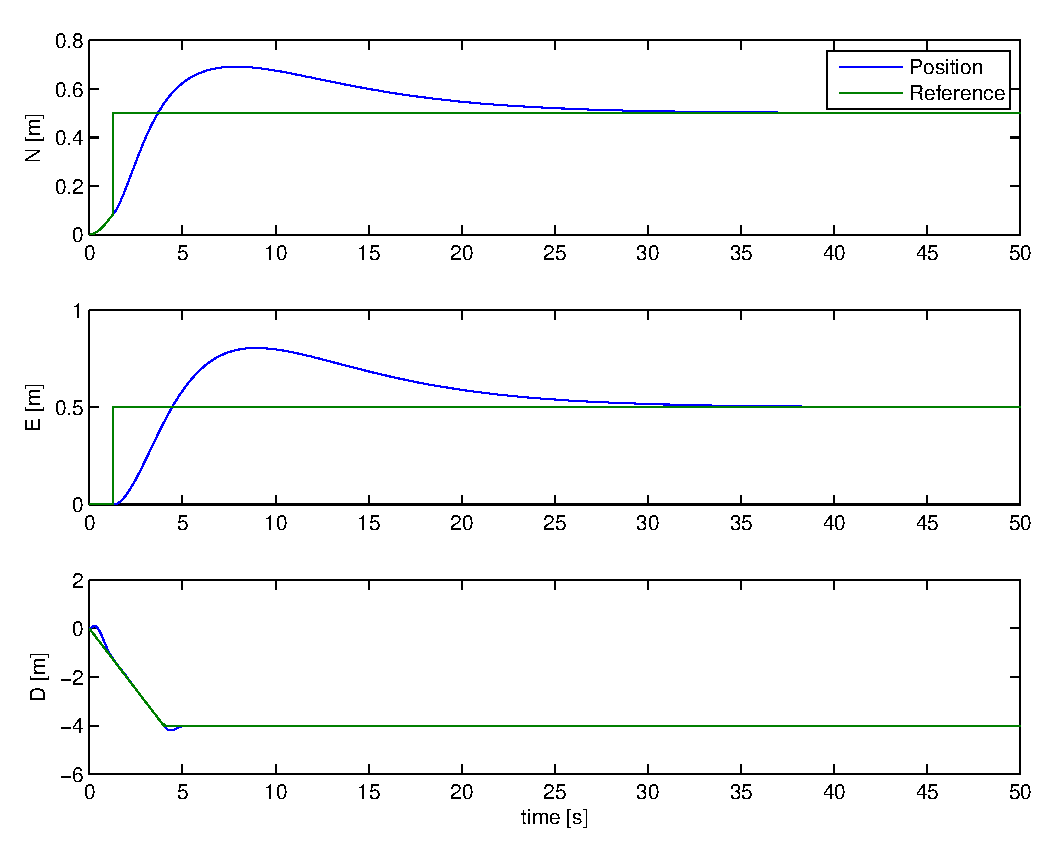
\includegraphics[width = 17cm]{fig/plots/simulation/positionNoDisturbance.eps}
\caption{Result}
\end{figure}
\subsubsection{Discussion}
\subsection{Simulation Without Constant Disturbances}
\subsubsection{Results}
\begin{figure}[H]
\centering
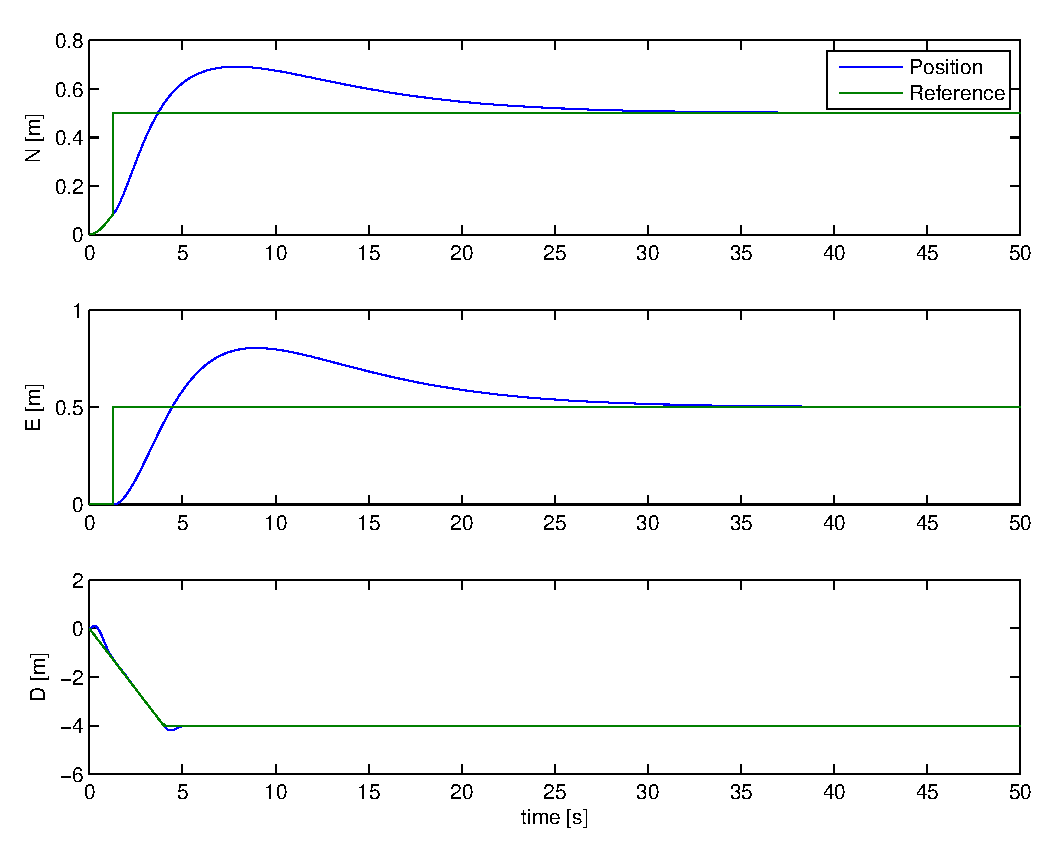
\includegraphics[width = 17cm]{fig/plots/simulation/positionNoDisturbance.eps}
\caption{Result}
\end{figure}
\subsubsection{Discussion}
\subsection{Simulation With Random Disturbances}
\subsubsection{Results}
\begin{figure}[H]
\centering
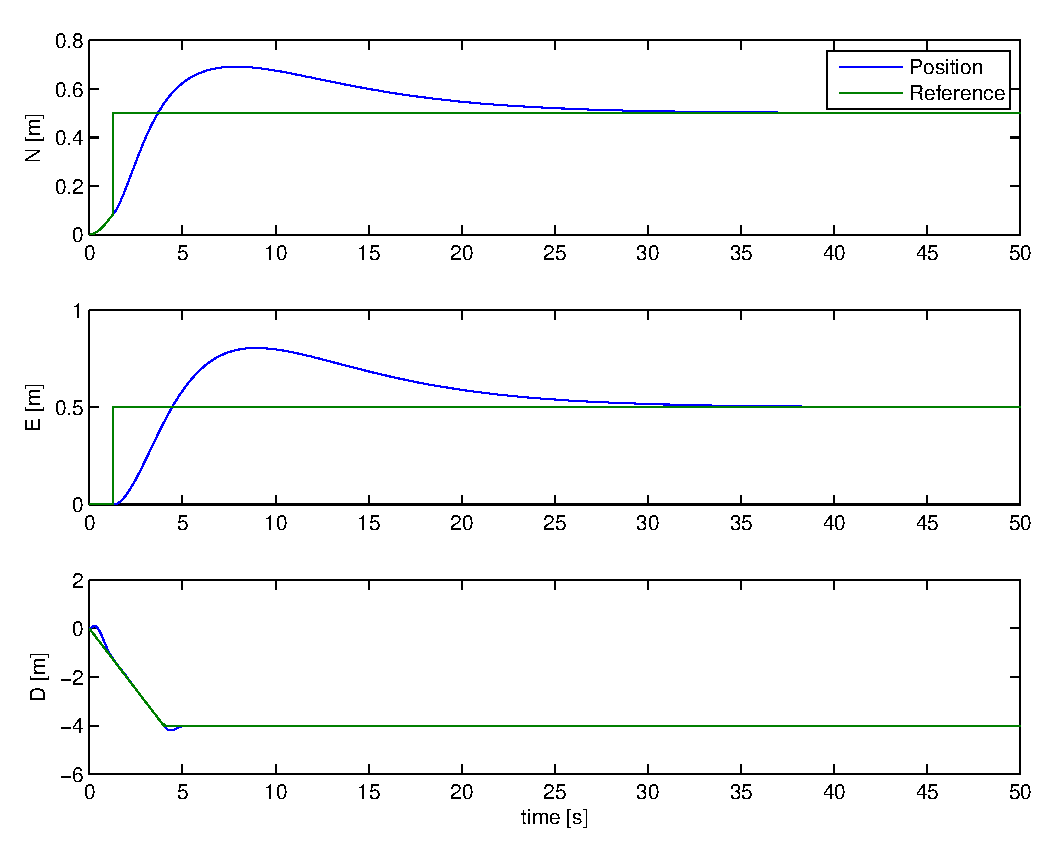
\includegraphics[width = 17cm]{fig/plots/simulation/positionNoDisturbance.eps}
\caption{Result}
\end{figure}
\begin{figure}[H]
\centering
\subfigure[Original image]{
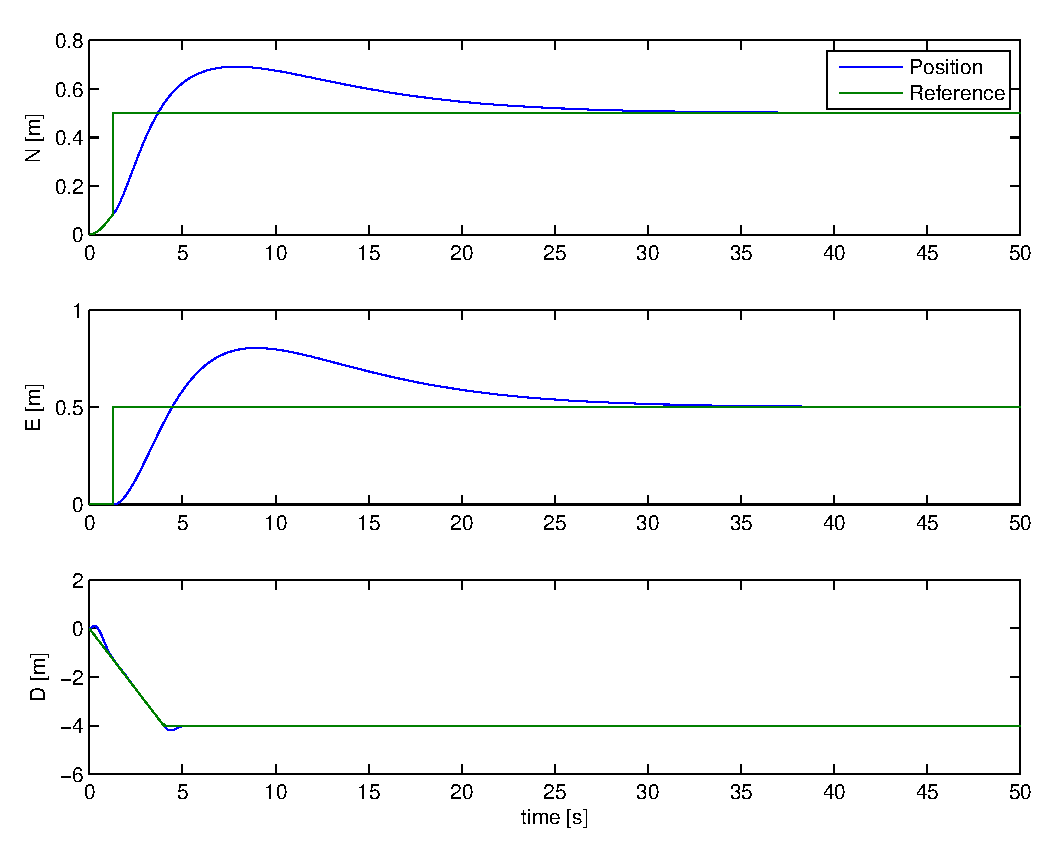
\includegraphics[width = 7cm]{fig/plots/simulation/positionNoDisturbance.eps}
}
\centering
\subfigure[HSV image]{
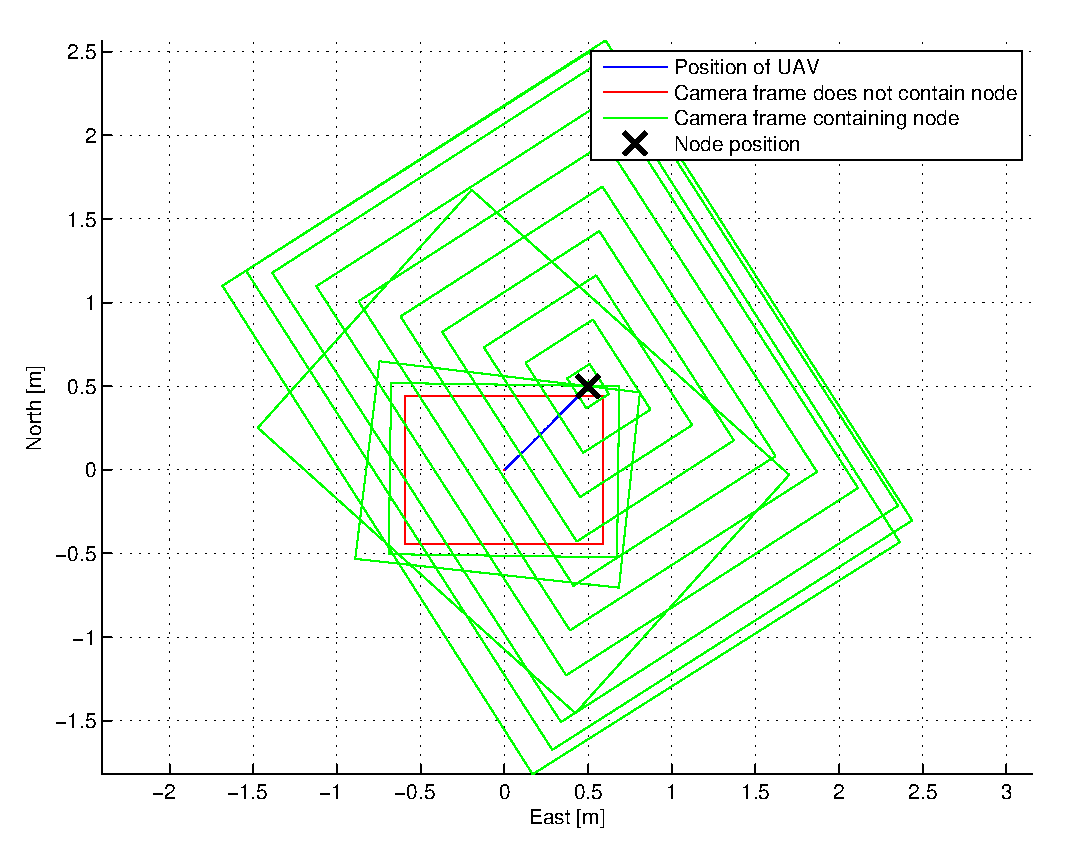
\includegraphics[width = 7cm]{fig/plots/simulation/positionFrameNoDisturbance.eps}
}
\caption{Results}
\end{figure}
\subsubsection{Discussion}